\documentclass[10pt]{article}
\usepackage[a4paper, margin=1in]{geometry}
\usepackage{amsmath}
\usepackage{booktabs}
\usepackage{xcolor}
\usepackage{listings}
\usepackage{hyperref}
\usepackage{tikz}
\usetikzlibrary{shapes.geometric, arrows.meta, positioning, matrix, fit, calc, decorations.pathreplacing}

% Define colors for code listings
\definecolor{codegreen}{rgb}{0,0.6,0}
\definecolor{codegray}{rgb}{0.5,0.5,0.5}
\definecolor{codepurple}{rgb}{0.58,0,0.82}
\definecolor{backcolour}{rgb}{0.95,0.95,0.92}

% Define a style for code listings
\lstdefinestyle{mystyle}{
    backgroundcolor=\color{backcolour},
    commentstyle=\color{codegreen},
    keywordstyle=\color{magenta},
    numberstyle=\tiny\color{codegray},
    stringstyle=\color{codepurple},
    basicstyle=\ttfamily\footnotesize,
    breakatwhitespace=false,
    breaklines=true,
    captionpos=b,
    keepspaces=true,
    numbers=left,
    numbersep=5pt,
    showspaces=false,
    showstringspaces=false,
    showtabs=false,
    tabsize=2
}

\lstset{style=mystyle}

% TikZ styles for diagrams
\tikzstyle{startstop} = [rectangle, rounded corners, minimum width=3cm, minimum height=1cm,text centered, draw=black, fill=red!30]
\tikzstyle{io} = [trapezium, trapezium left angle=70, trapezium right angle=110, minimum width=3cm, minimum height=1cm, text centered, draw=black, fill=blue!30]
\tikzstyle{process} = [rectangle, minimum width=3cm, minimum height=1cm, text centered, draw=black, fill=orange!30]
\tikzstyle{decision} = [diamond, minimum width=3cm, minimum height=1cm, text centered, draw=black, fill=green!30]
\tikzstyle{arrow} = [thick,->,>=stealth]
\tikzstyle{block} = [rectangle, draw, fill=blue!20, text width=6em, text centered, rounded corners, minimum height=4em]
\tikzstyle{line} = [draw, -latex']
\tikzstyle{mem} = [rectangle, draw, minimum width=2cm, minimum height=1cm, text centered]
\tikzstyle{level} = [rectangle, draw, fill=blue!20, minimum width=6cm, text centered]


\title{COMP2130 Cheat Sheet}
\author{}
\date{}

\begin{document}

\maketitle

\section{Week 1: Machine-Level Programming I: Basics}

\subsection{History of Intel Processors and Architectures}
\begin{itemize}
    \item \textbf{Intel x86 Processors:} Dominant in the PC market, featuring a backward-compatible, evolutionary design. They are Complex Instruction Set Computers (CISC).
    \item \textbf{Milestones:}
    \begin{itemize}
        \item \textbf{8086 (1978):} 16-bit processor, basis for IBM PC/DOS.
        \item \textbf{386 (1985):} First 32-bit (IA32) processor.
        \item \textbf{Pentium 4E (2004):} First 64-bit (x86-64) processor.
        \item \textbf{Core 2 (2006):} First multi-core processor.
        \item \textbf{Core i7 (2008):} Four cores, integrated memory controller.
    \end{itemize}
    \item \textbf{AMD:} Competitor to Intel, developed x86-64.
\end{itemize}

\subsection{C, Assembly, and Machine Code}
The compilation process transforms human-readable C code into machine-executable code.
\begin{figure}[h]
    \centering
    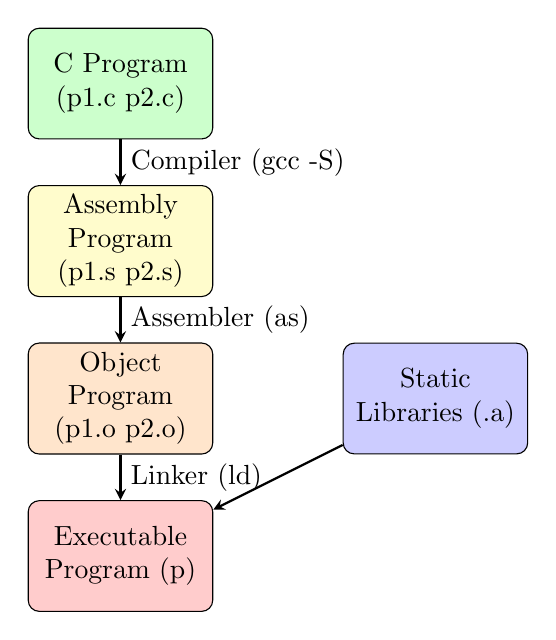
\begin{tikzpicture}[node distance=2cm]
        \node (c_code) [block, fill=green!20] {C Program (p1.c p2.c)};
        \node (asm_code) [block, fill=yellow!20, below of=c_code] {Assembly Program (p1.s p2.s)};
        \node (obj_code) [block, fill=orange!20, below of=asm_code] {Object Program (p1.o p2.o)};
        \node (exe_code) [block, fill=red!20, below of=obj_code] {Executable Program (p)};
        \node (libs) [block, fill=blue!20, right of=obj_code, xshift=2cm] {Static Libraries (.a)};

        \draw [arrow] (c_code) -- node[anchor=west] {Compiler (gcc -S)} (asm_code);
        \draw [arrow] (asm_code) -- node[anchor=west] {Assembler (as)} (obj_code);
        \draw [arrow] (obj_code) -- node[anchor=west] {Linker (ld)} (exe_code);
        \draw [arrow] (libs) -- (exe_code);
    \end{tikzpicture}
    \caption{Compilation Process}
\end{figure}

\subsection{Assembly Basics}
\begin{table}[h]
    \centering
    \caption{x86-64 Registers}
    \begin{tabular}{ll}
        \toprule
        Register & Use \\
        \midrule
        \%rax & Return value \\
        \%rdi, \%rsi, \%rdx, \%rcx, \%r8, \%r9 & First 6 function arguments \\
        \%rsp & Stack pointer \\
        \bottomrule
    \end{tabular}
\end{table}

\subsubsection{Addressing Modes}
\begin{lstlisting}[language=c]
// Immediate: Constant integer data
movq $0x4, %rax //

// Register: One of 16 integer registers
movq %rax, %rdx //

// Memory: 8 consecutive bytes of memory at address
movq (%rax), %rdx //
\end{lstlisting}

\subsection{Arithmetic \& Logical Operations}
\begin{table}[h]
    \centering
    \caption{Common Arithmetic and Logical Instructions}
    \begin{tabular}{ll}
        \toprule
        Instruction & Description \\
        \midrule
        \texttt{leaq Src, Dst} & Load Effective Address \\
        \texttt{addq Src, Dst} & Add \\
        \texttt{subq Src, Dst} & Subtract \\
        \texttt{imulq Src, Dst} & Multiply \\
        \texttt{salq Src, Dst} & Left Shift \\
        \texttt{sarq Src, Dst} & Arithmetic Right Shift \\
        \texttt{shrq Src, Dst} & Logical Right Shift \\
        \texttt{xorq Src, Dst} & Exclusive OR \\
        \texttt{andq Src, Dst} & And \\
        \texttt{orq Src, Dst} & Or \\
        \bottomrule
    \end{tabular}
\end{table}

\section{Week 2: Machine-Level Programming II, III, \& IV}

\subsection{Control Flow}
\begin{itemize}
    \item \textbf{Condition Codes:} Single-bit registers set by arithmetic/logical operations.
    \begin{itemize}
        \item CF: Carry Flag
        \item ZF: Zero Flag
        \item SF: Sign Flag
        \item OF: Overflow Flag
    \end{itemize}
    \item \textbf{Instructions:}
    \begin{itemize}
        \item \texttt{cmpq Src2, Src1}: Sets condition codes based on \texttt{Src1 - Src2}.
        \item \texttt{testq Src2, Src1}: Sets condition codes based on \texttt{Src1 \& Src2}.
        \item \texttt{setX}: Sets a byte based on condition codes.
        \item \texttt{jX}: Jumps based on condition codes.
    \end{itemize}
\end{itemize}

\subsection{Procedures}
\begin{figure}[h]
    \centering
    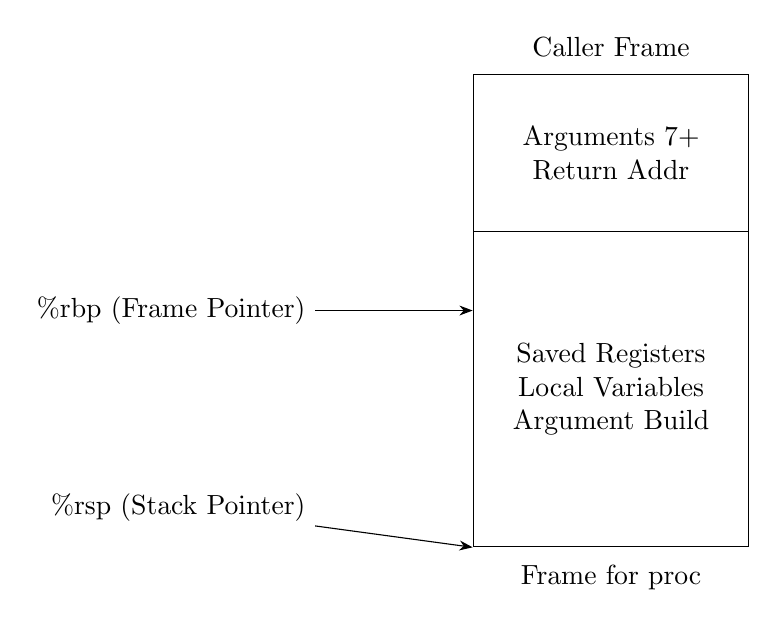
\begin{tikzpicture}[
        node distance=0cm,
        frame/.style={draw, minimum width=3.5cm, align=center}
    ]
        % Define the stack frames vertically
        \node (caller) [frame, minimum height=2cm] at (0, 3) {Arguments 7+\\Return Addr};
        \node (callee) [frame, minimum height=4cm] at (0, 0) {Saved Registers\\Local Variables\\Argument Build};

        % Add labels
        \node[above=0.1cm of caller] {Caller Frame};
        \node[below=0.1cm of callee] {Frame for proc};
        
        % Add pointers
        \node (rbp_label) [left=2cm of callee, yshift=1cm] {\%rbp (Frame Pointer)};
        \draw[-Stealth] (rbp_label) -- (callee.west |- rbp_label);

        \node (rsp_label) [left=2cm of callee, yshift=-1.5cm] {\%rsp (Stack Pointer)};
        \draw[-Stealth] (rsp_label) -- (callee.south west);

    \end{tikzpicture}   
    \caption{Stack Frame}
\end{figure}
\begin{itemize}
    \item \textbf{Stack Frame:} A region on the stack for a single procedure call.
    \item \textbf{Control Transfer:}
    \begin{itemize}
        \item \texttt{call label}: Pushes return address, jumps to \texttt{label}.
        \item \texttt{ret}: Pops return address, jumps to it.
    \end{itemize}
    \item \textbf{Register Saving Conventions:}
    \begin{itemize}
        \item \textbf{Caller-saved:} \%rax, \%rdi-\%r9, \%r10, \%r11
        \item \textbf{Callee-saved:} \%rbx, \%r12-\%r14, \%rbp, \%rsp
    \end{itemize}
\end{itemize}

\subsection{Data}
\begin{itemize}
    \item \textbf{Arrays:} Contiguous memory blocks.
    \begin{itemize}
        \item 1D: \texttt{T A[L]}
        \item 2D: \texttt{T A[R][C]} (row-major order)
    \end{itemize}
    \item \textbf{Structs:} Memory block holding all fields, with padding for alignment.
\end{itemize}
\begin{figure}[h]
    \centering
    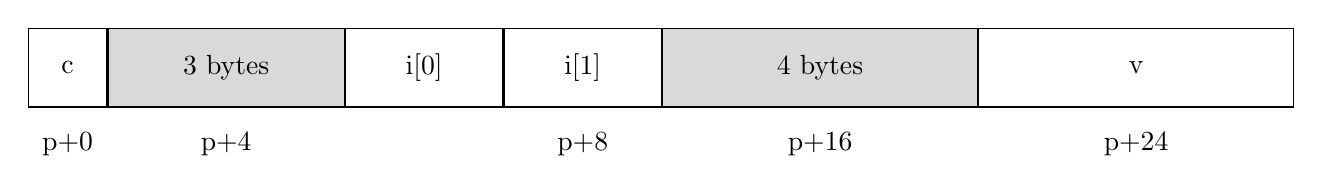
\begin{tikzpicture}[node distance=0cm]
        \node (c) [mem, minimum width=1cm] {c};
        \node (pad1) [mem, fill=gray!30, right=of c, minimum width=3cm] {3 bytes};
        \node (i0) [mem, right=of pad1, minimum width=2cm] {i[0]};
        \node (i1) [mem, right=of i0, minimum width=2cm] {i[1]};
        \node (pad2) [mem, fill=gray!30, right=of i1, minimum width=4cm] {4 bytes};
        \node (v) [mem, right=of pad2, minimum width=4cm] {v};
        
        \node[below=0.2cm of c] {p+0};
        \node[below=0.2cm of pad1] {p+4};
        \node[below=0.2cm of i0] {}; % Adjusted for spacing
        \node[below=0.2cm of i1] {p+8};
        \node[below=0.2cm of pad2] {p+16};
        \node[below=0.2cm of v] {p+24};
    \end{tikzpicture}
    \caption{Struct Alignment}
\end{figure}

\section{Week 3: Linking, Advanced Topics, and Optimization}

\subsection{Linking}
\begin{figure}[h]
    \centering
    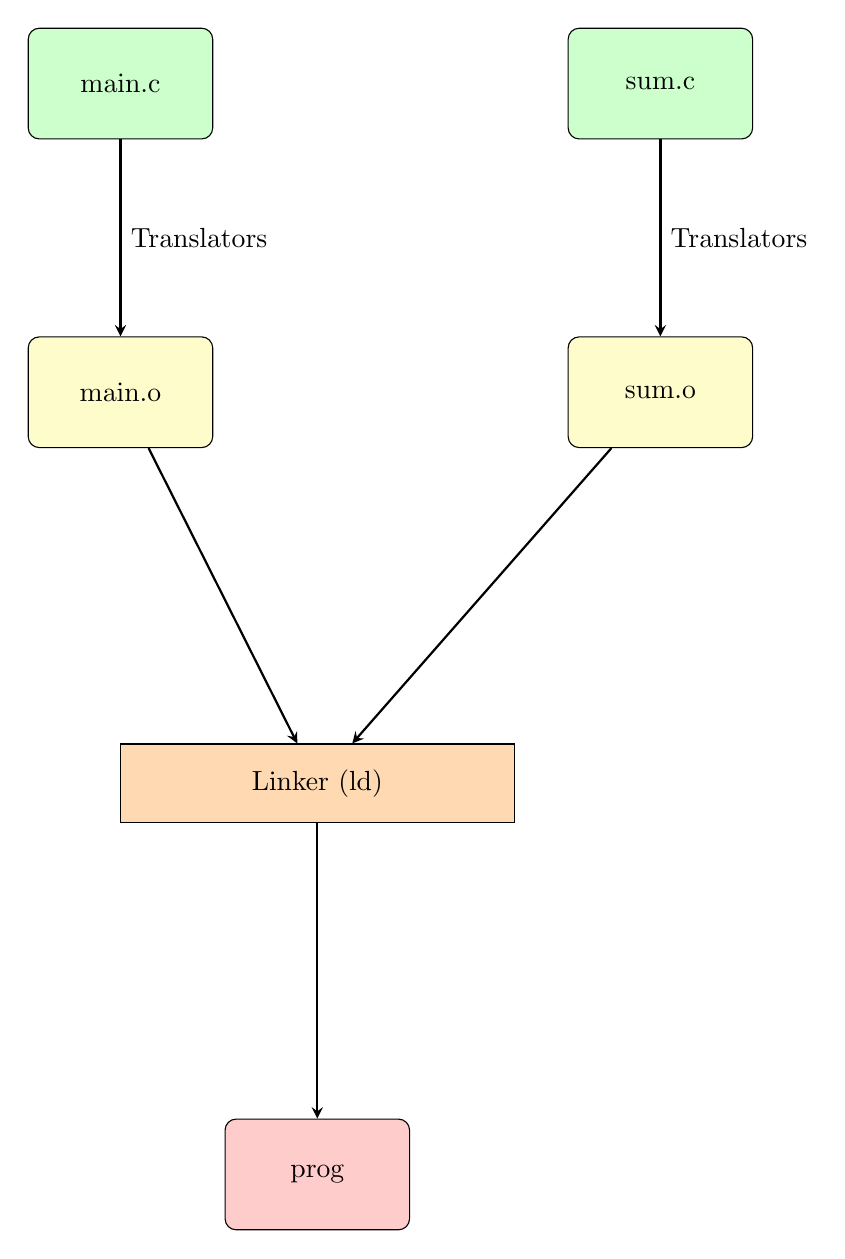
\begin{tikzpicture}[node distance=2.5cm, auto]
        \node (main_c) [block, fill=green!20] {main.c};
        \node (sum_c) [block, fill=green!20, right=of main_c, xshift=2cm] {sum.c};
        \node (main_o) [block, fill=yellow!20, below=of main_c] {main.o};
        \node (sum_o) [block, fill=yellow!20, below=of sum_c] {sum.o};
        \node (linker) [process, below=of main_o, yshift=-1.25cm, xshift=2.5cm, minimum width=5cm] {Linker (ld)};
        \node (prog) [block, fill=red!20, below=of linker, yshift=-1.25cm] {prog};
        
        \draw[arrow] (main_c) -- node[midway, right] {Translators} (main_o);
        \draw[arrow] (sum_c) -- node[midway, right] {Translators} (sum_o);
        \draw[arrow] (main_o) -- (linker);
        \draw[arrow] (sum_o) -- (linker);
        \draw[arrow] (linker) -- (prog);
    \end{tikzpicture}
    \caption{Linking Process}
\end{figure}

\subsection{Advanced Topics}
\begin{itemize}
    \item \textbf{Memory Layout:} Stack, Heap, Data, Text.
    \item \textbf{Buffer Overflow:} Writing data beyond a buffer's boundaries, a major security vulnerability.
    \item \textbf{Unions:} Data structures that store different data types in the same memory location.
\end{itemize}
\begin{figure}[h!]
    \centering
    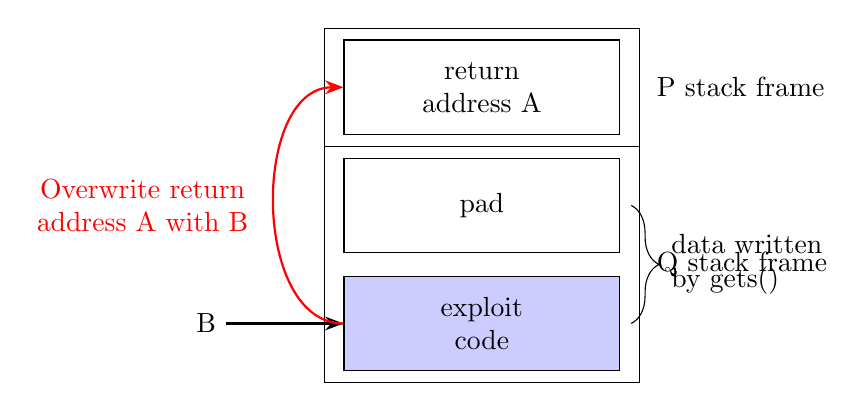
\begin{tikzpicture}[
        % Define a style for the boxes inside the stack
        stack_box/.style={draw, minimum width=3.5cm, minimum height=1.2cm, align=center}
    ]
        % --- Draw the stack elements at fixed positions ---
        \node (ret_addr) [stack_box] at (0, 3) {return\\address A};
        \node (pad)      [stack_box] at (0, 1.5) {pad};
        \node (exploit)  [stack_box, fill=blue!20] at (0, 0) {exploit\\code};

        % --- Draw the outer frame boxes at fixed positions ---
        \draw (-2, 2.25) rectangle (2, 3.75);
        \node[right] at (2.1, 3) {P stack frame};

        \draw (-2, -0.75) rectangle (2, 2.25);
        \node[right] at (2.1, 0.75) {Q stack frame};
        
        % --- Add labels and arrows at fixed positions ---
        \node (b_label) at (-3.5, 0) {B};
        \draw[-Stealth, thick] (b_label) -- (exploit.west);

        \draw[-Stealth, red, thick, out=180, in=180]
            (exploit.west) to node[left=0.2cm, align=center] {Overwrite return\\address A with B} (ret_addr.west);

        % --- Draw the brace and its label ---
        \draw[decorate, decoration={brace, amplitude=10pt, mirror, raise=4pt}]
            (exploit.east) -- (pad.east) 
            node[midway, right, xshift=15pt, align=left] {data written\\by gets()};

    \end{tikzpicture}
    \caption{Buffer Overflow Attack}
\end{figure}



\subsection{Optimization}
\begin{itemize}
    \item \textbf{Constant Folding:} Compile-time evaluation of constant expressions.
    \item \textbf{Dead Code Elimination:} Removing unreachable code.
    \item \textbf{Common Subexpression Elimination:} Reusing results of computations.
    \item \textbf{Code Motion:} Moving loop-invariant code out of loops.
    \item \textbf{Inlining:} Replacing function calls with the function's body.
\end{itemize}

\section{Week 4: ECF and Memory Hierarchy}

\subsection{Exceptional Control Flow (ECF)}
\begin{itemize}
    \item \textbf{Exceptions:} Transfer of control to the OS.
    \item \textbf{Processes:} Instances of running programs.
    \item \textbf{Signals:} Messages notifying a process of an event.
\end{itemize}
\begin{figure}[h]
    \centering
    \begin{tikzpicture}[>=Stealth]
        % Timeline arrow
        \draw[->, very thick] (0,5) -> (0,0) node[below] {Time};

        % Process flows with labels
        \node (pA_label) at (1.5, 5) {Process A};
        \draw[thick] (pA_label.south) -- +(0,-1);
        \draw[thick, red] (pA_label.south) ++(0,-1) -- +(0,-1);
        \draw[thick] (pA_label.south) ++(0,-2) -- +(0,-1);
        \draw[thick, red] (pA_label.south) ++(0,-3) -- +(0,-1);

        \node (pB_label) [right=1.5cm of pA_label] {Process B};
        \draw[thick, yellow!80!black] (pB_label.south) ++(0,-0.5) -- +(0,-0.5);

        \node (pC_label) [right=1.5cm of pB_label] {Process C};
        \draw[thick, red] (pC_label.south) ++(0,-1.5) -- +(0,-0.5);
        \draw[thick, red] (pC_label.south) ++(0,-3.5) -- +(0,-0.5);

    \end{tikzpicture}
    \caption{Concurrent Process Execution}
\end{figure}

\subsection{The Memory Hierarchy}
\begin{itemize}
    \item \textbf{Locality:}
    \begin{itemize}
        \item \textbf{Temporal:} Recently accessed items are likely to be accessed again.
        \item \textbf{Spatial:} Items with nearby addresses are likely to be accessed together.
    \end{itemize}
    \item \textbf{Caching:} Using a smaller, faster memory to store a subset of data from a larger, slower memory.
\end{itemize}
\begin{figure}[h]
    \centering
    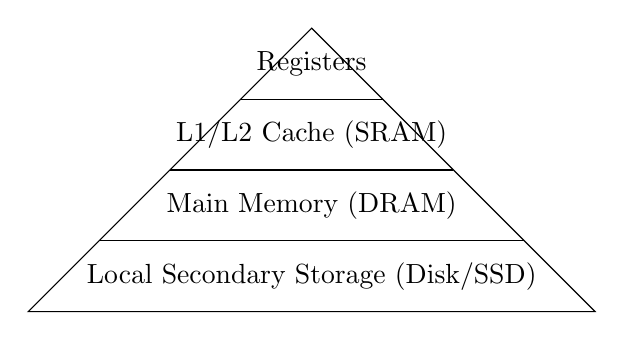
\begin{tikzpicture}[scale=0.9]
        \draw (0,0) -- (4,4) -- (8,0) -- cycle;
        \node at (4,3.5) {Registers};
        \draw (3,3) -- (5,3);
        \node at (4,2.5) {L1/L2 Cache (SRAM)};
        \draw (2,2) -- (6,2);
        \node at (4,1.5) {Main Memory (DRAM)};
        \draw (1,1) -- (7,1);
        \node at (4,0.5) {Local Secondary Storage (Disk/SSD)};
    \end{tikzpicture}
    \caption{Memory Hierarchy}
\end{figure}

\section{Week 5: Virtual Memory}

\subsection{Virtual Memory (VM)}
\begin{itemize}
    \item \textbf{Address Spaces:} Virtual (program's view) and Physical (hardware's view).
    \item \textbf{Page Table:} Maps virtual pages to physical pages.
    \item \textbf{Page Fault:} An exception that occurs when a program accesses a page that is not in physical memory.
    \item \textbf{Address Translation:} The process of converting a virtual address to a physical address.
\end{itemize}
\begin{figure}[h]
    \centering
    % The 'scale' option is a better way to resize TikZ diagrams
    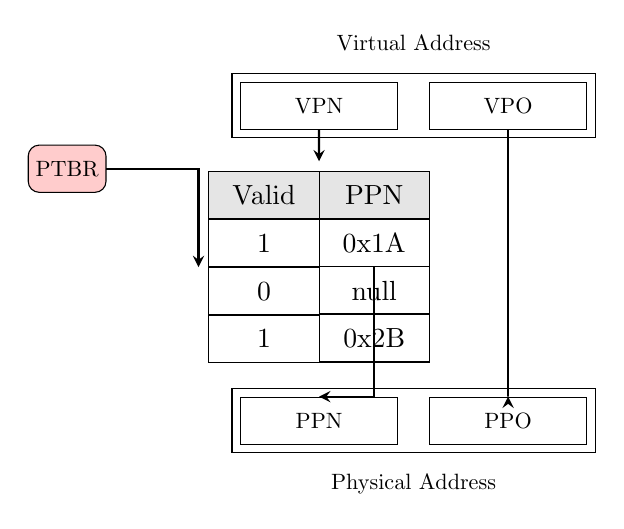
\begin{tikzpicture}[scale=0.8, transform shape, node distance=1.5cm and 1cm, >=Stealth]
        % Top Layer: Virtual Address
        \node (va_label) at (3.5, 3) {Virtual Address};
        \node (vpn) [draw, minimum width=2.5cm, minimum height=0.75cm] at (2,2) {VPN};
        \node (vpo) [draw, minimum width=2.5cm, minimum height=0.75cm] at (5,2) {VPO};
        % Use a 'fit' node to draw the outer box without filling
        \node[fit=(vpn)(vpo), draw, inner sep=0.1cm] (va_box) {};

        % Middle Layer: Page Table
        \node (ptbr) [draw, rounded corners, fill=red!20, minimum height=0.75cm] at (-2,1) {PTBR};
        \node (pt) [matrix of nodes, below=0.5cm of vpn,
            nodes={draw, minimum width=1.4cm, minimum height=0.6cm},
            row sep=-\pgflinewidth, column sep=-\pgflinewidth]
        {
            \node[fill=gray!20]{Valid}; & \node[fill=gray!20]{PPN}; \\
            1 & 0x1A \\
            0 & null \\
            1 & 0x2B \\
        };
        
        % Bottom Layer: Physical Address
        \node (pa_label) at (3.5, -4) {Physical Address};
        \node (ppn) [draw, minimum width=2.5cm, minimum height=0.75cm] at (2,-3) {PPN};
        \node (ppo) [draw, minimum width=2.5cm, minimum height=0.75cm] at (5,-3) {PPO};
        % Use a 'fit' node for the outer box
        \node[fit=(ppn)(ppo), draw, inner sep=0.1cm] (pa_box) {};

        % Arrows
        \draw[arrow] (ptbr.east) -| (pt.west);
        \draw[arrow] (vpn.south) -- (pt.north);
        \draw[arrow] (vpo.south) |- (ppo.north);
        \draw[arrow] (pt-2-2.south) |- (ppn.north);
    \end{tikzpicture}
    \caption{Address Translation}
\end{figure}

\end{document}